\documentclass[
size=17pt,
paper=smartboard,
mode=present,
display=slidesnotes,
style=paintings,
nopagebreaks,
blackslide,
fleqn]{powerdot}

% styles: sailor, paintings
% wj capsules prettybox
% mode = handout or present


\newcommand{\palette}{Moitessier}
% palettes:
%    - sailor: Sea, River, Wine, Chocolate, Cocktail 
%    - paintings: Syndics, Skater, GoldenGate, Moitessier, PearlEarring, Lamentation, HolyWood, Europa, MayThird, Charon 

\newcommand{\cursopequeno}{EC01045 PDS}
\newcommand{\cursogrande}{\Large EC01045 -- Processamento digital de sinais}

\usepackage{amsmath,graphicx,color,amsfonts}
\usepackage[brazilian]{babel}
\usepackage[utf8]{inputenc}
\usepackage{bbding}

\author{Ronaldo de Freitas Zampolo\\FCT-ITEC-UFPA}
\date{ERE 2020}


\pdsetup{
   lf = {\cursopequeno},
   rf = {Estruturas de implementação},
   palette = \palette,randomdots={false},
   cf={\theslide}
}

\title{\cursogrande\\ \vspace{1cm}Estruturas de implementação}

\begin{document}
\maketitle[randomdots={false}]
   \begin{slide}{Agenda}
      \tableofcontents[content=sections]
   \end{slide}


\section{Introdução}
%\begin{slide}{T\'opicos}
%\begin{itemize}
%  \item Introdu\c c\~ao
%  \item Representação em diagrama de blocos
%  \item Representa\c c\~ao em grafos de fluxo de sinal
%  \item Estruturas básicas
%  \item Formas transpostas
%\end{itemize}
%\end{slide}

\begin{slide}{Introdu\c c\~ao}
\begin{itemize}
   \item Representações equivalentes de um sistema linear e invariante
   \begin{figure}
      \centering
      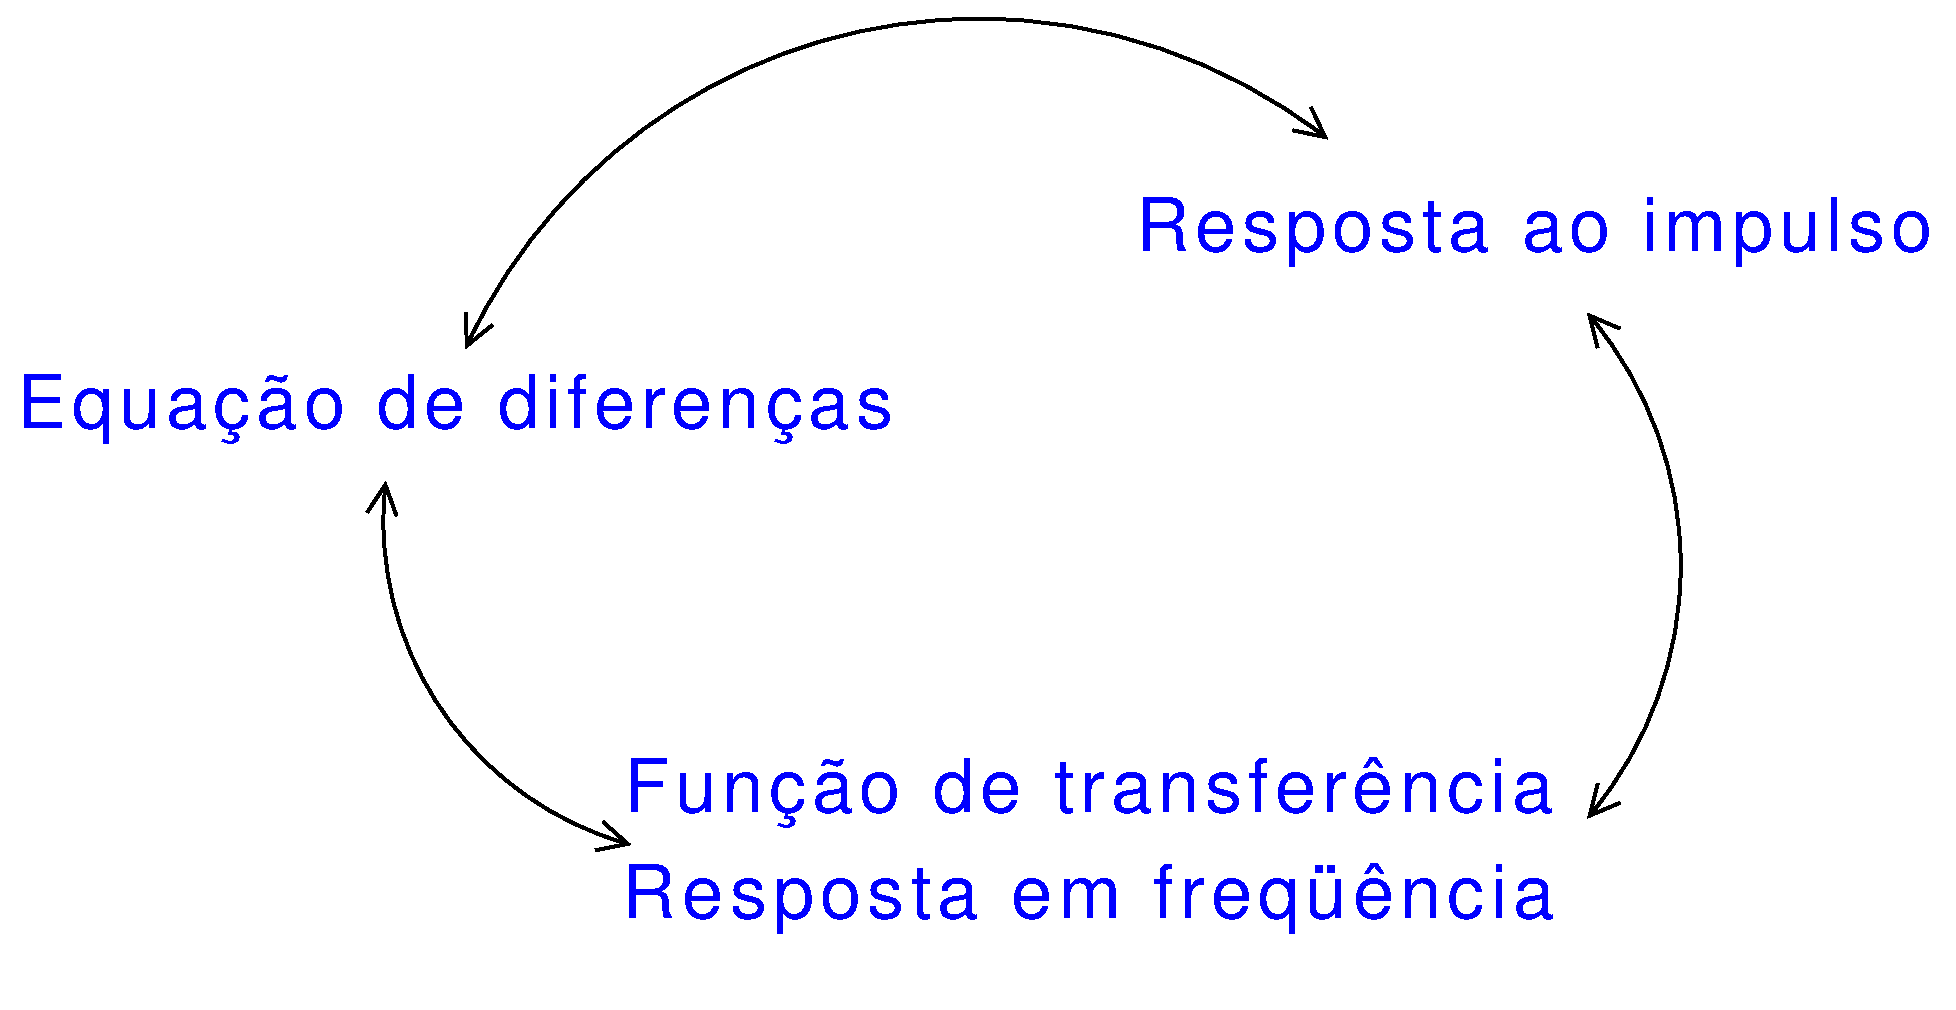
\includegraphics[width = 0.8\textwidth]{figs/Estrut_intro01.eps}
   \end{figure}
\end{itemize}
\end{slide}

%\overlays{3}{
\begin{slide}{Introdu\c c\~ao}
\begin{itemize}
   \item Ex.: Ache a resposta ao impulso e a eq. de diferenças a partir da função de transferência
   \begin{equation*}
      H(z)=\frac{b_0 + b_1z^{-1}}{1-az^{-1}}, \qquad |z|>|a|
   \end{equation*}
   %\fromSlide{2}{
   \begin{equation*}
      h[n]=b_0a^nu[n] + b_1a^{n-1}u[n-1]
   \end{equation*}%}
   %\fromSlide{3}{
   \begin{equation*}
      y[n]-ay[n-1]=b_0x[n] + b_1x[n-1]
   \end{equation*}%}
\end{itemize}
\end{slide}%}

\begin{slide}{Introdu\c c\~ao}
\begin{itemize}
   \item Ex.: (Continuação)
   \begin{align*}
      H(z) &= \frac{b_0 + b_1z^{-1}}{1-az^{-1}}, \qquad |z|>|a| \\
      a &= -0,9\qquad b_0=0,5\qquad b_1=1
   \end{align*}
   \begin{figure}
      \centering
      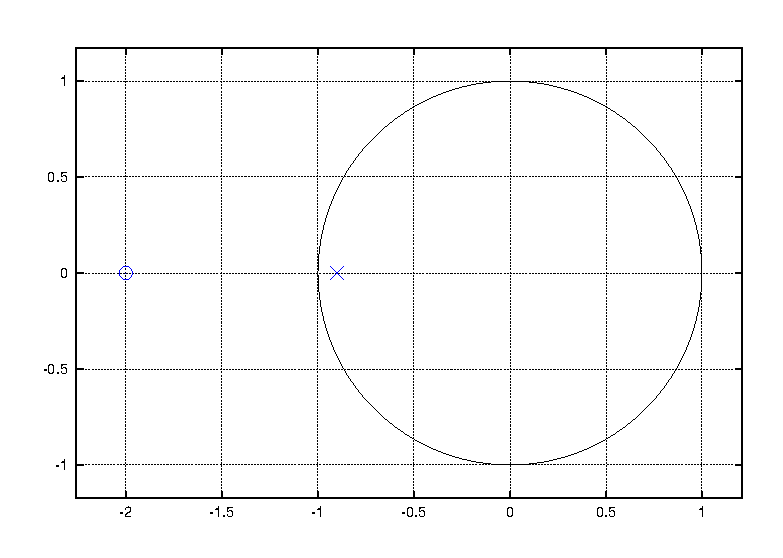
\includegraphics[width = 0.45\textwidth]{figs/pol_zer1.eps}
      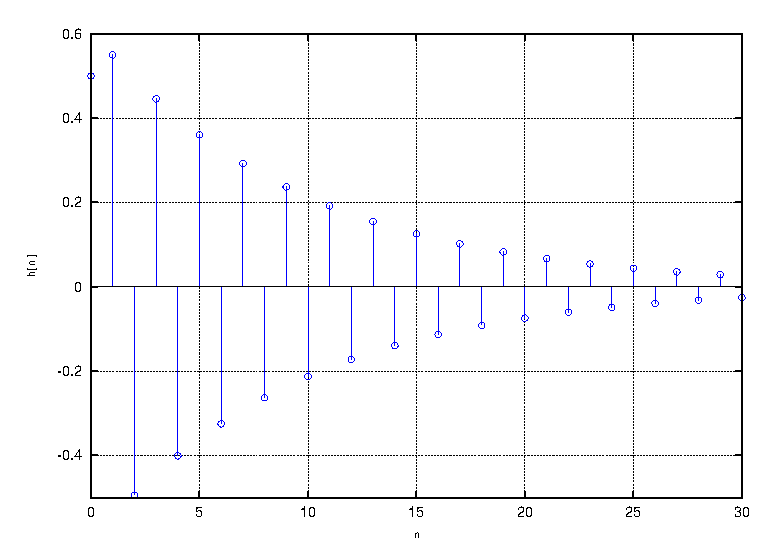
\includegraphics[width = 0.45\textwidth]{figs/imp_resp1.eps}
   \end{figure}
\end{itemize}
\end{slide}

\begin{slide}{Introdu\c c\~ao}
\begin{itemize}
   \item Ex.: (Continuação)
   \begin{align*}
      H(z) &= \frac{b_0 + b_1z^{-1}}{1-az^{-1}}, \qquad |z|>|a| \\
      a &= -0,9\qquad b_0=0,5\qquad b_1=1
   \end{align*}
   \begin{figure}
      \centering
      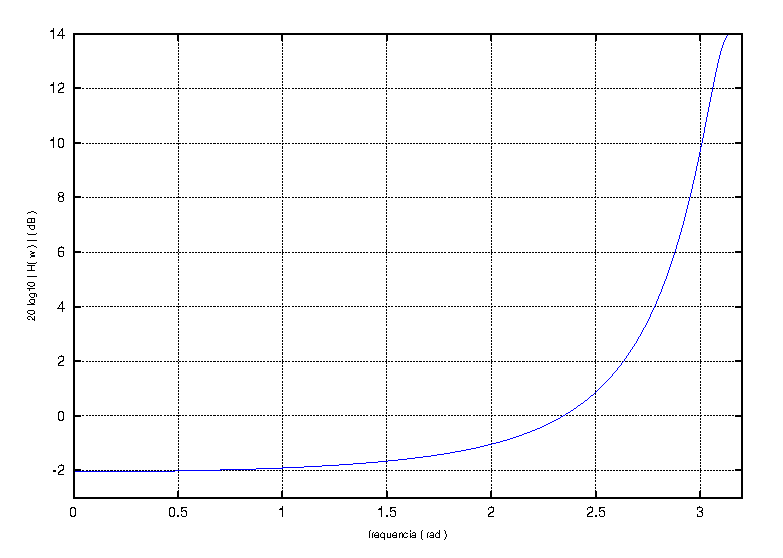
\includegraphics[width = 0.45\textwidth]{figs/mod1.eps}
      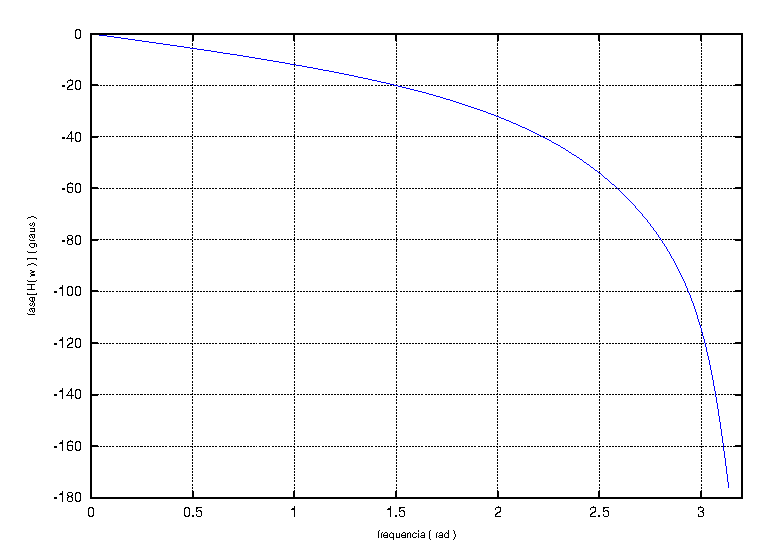
\includegraphics[width = 0.45\textwidth]{figs/fase1.eps}
   \end{figure}
\end{itemize}
\end{slide}

\begin{slide}{Introdu\c c\~ao}
\begin{itemize}
   \item Ex.: (Continuação)
   \begin{align*}
      H(z) &= \frac{b_0 + b_1z^{-1}}{1-az^{-1}}, \qquad |z|>|a| \\
      a &= -1,1\qquad b_0=0,5\qquad b_1=1
   \end{align*}
   \begin{figure}
      \centering
      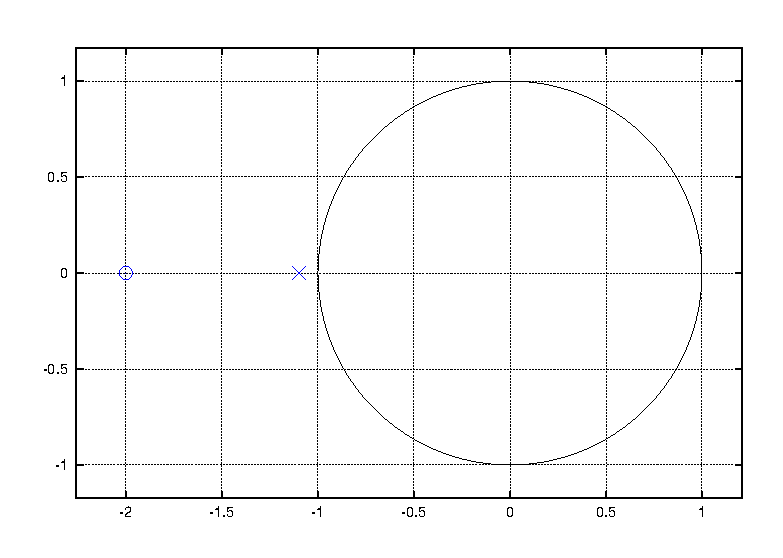
\includegraphics[width = 0.45\textwidth]{figs/pol_zer2.eps}
      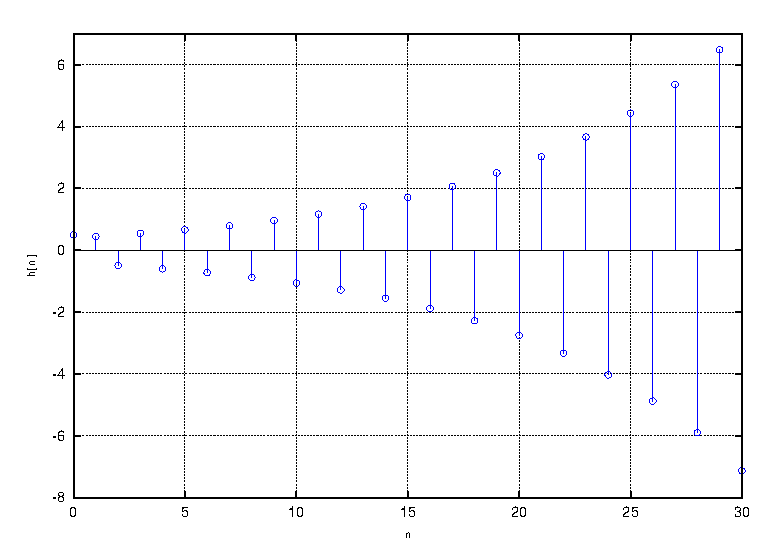
\includegraphics[width = 0.45\textwidth]{figs/imp_resp2.eps}
   \end{figure}
\end{itemize}
\end{slide}

\section{Representação em diagrama de blocos}
\begin{slide}{Diagrama de blocos}
\begin{itemize}
   \item Elementos básicos
   \begin{itemize}
      \item Soma
       \begin{figure}
          \centering
          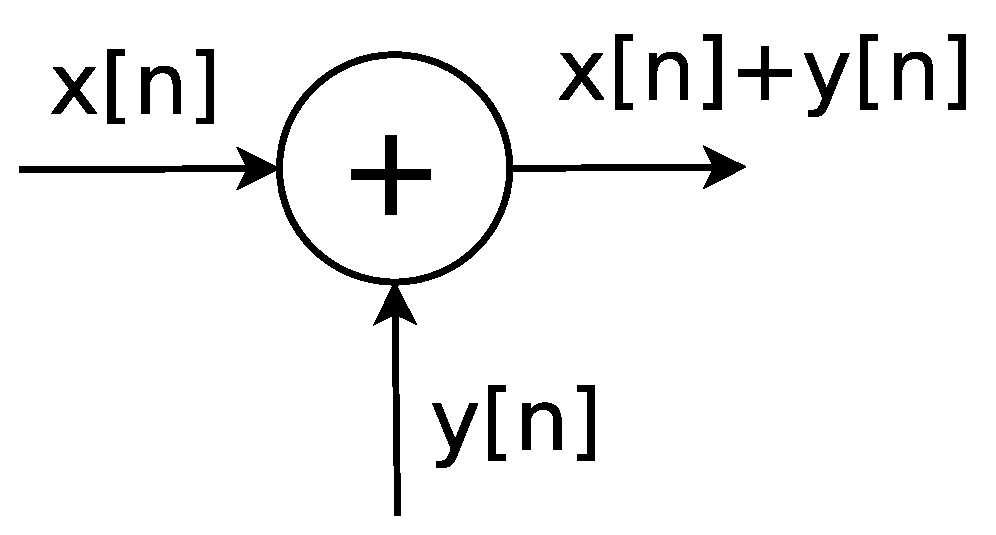
\includegraphics[width = 0.3\textwidth]{figs/soma.eps}
       \end{figure}
      \item Multiplicação
      \begin{figure}
          \centering
          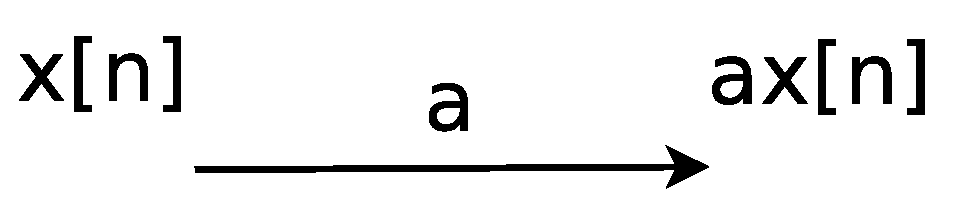
\includegraphics[width = 0.3\textwidth]{figs/mult.eps}
       \end{figure}
      \item Atraso
       \begin{figure}
          \centering
          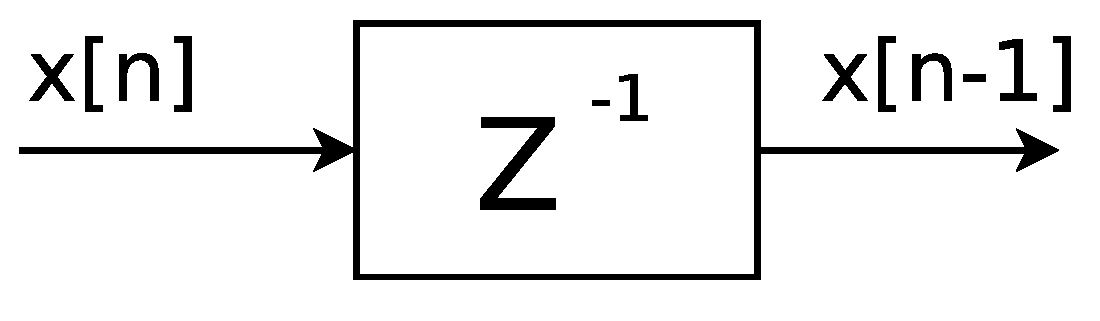
\includegraphics[width = 0.3\textwidth]{figs/atraso.eps}
       \end{figure}
    \end{itemize}
\end{itemize}
\end{slide}

\begin{slide}{Diagrama de blocos}
\begin{itemize}
   \item Ex.: represente em diagrama de blocos a eq. de diferenças do exemplo anterior
    \begin{equation*}
        y[n] -ay[n-1]= b_0x[n]+b_1x[n-1] 
    \end{equation*}
   \item Ex.: represente em diagrama de blocos a eq. de diferenças 
   \begin{equation*}
        y[n]= a_1y[n-1]+a_2y[n-2]+b_0x[n] 
    \end{equation*}
\end{itemize}
\end{slide}

\begin{slide}{Diagrama de blocos}
\begin{itemize}
     \item Continuação
      \begin{equation*}
        y[n]= a_1y[n-1]+a_2y[n-2]+b_0x[n] 
    \end{equation*}
   \begin{figure}
       \centering
        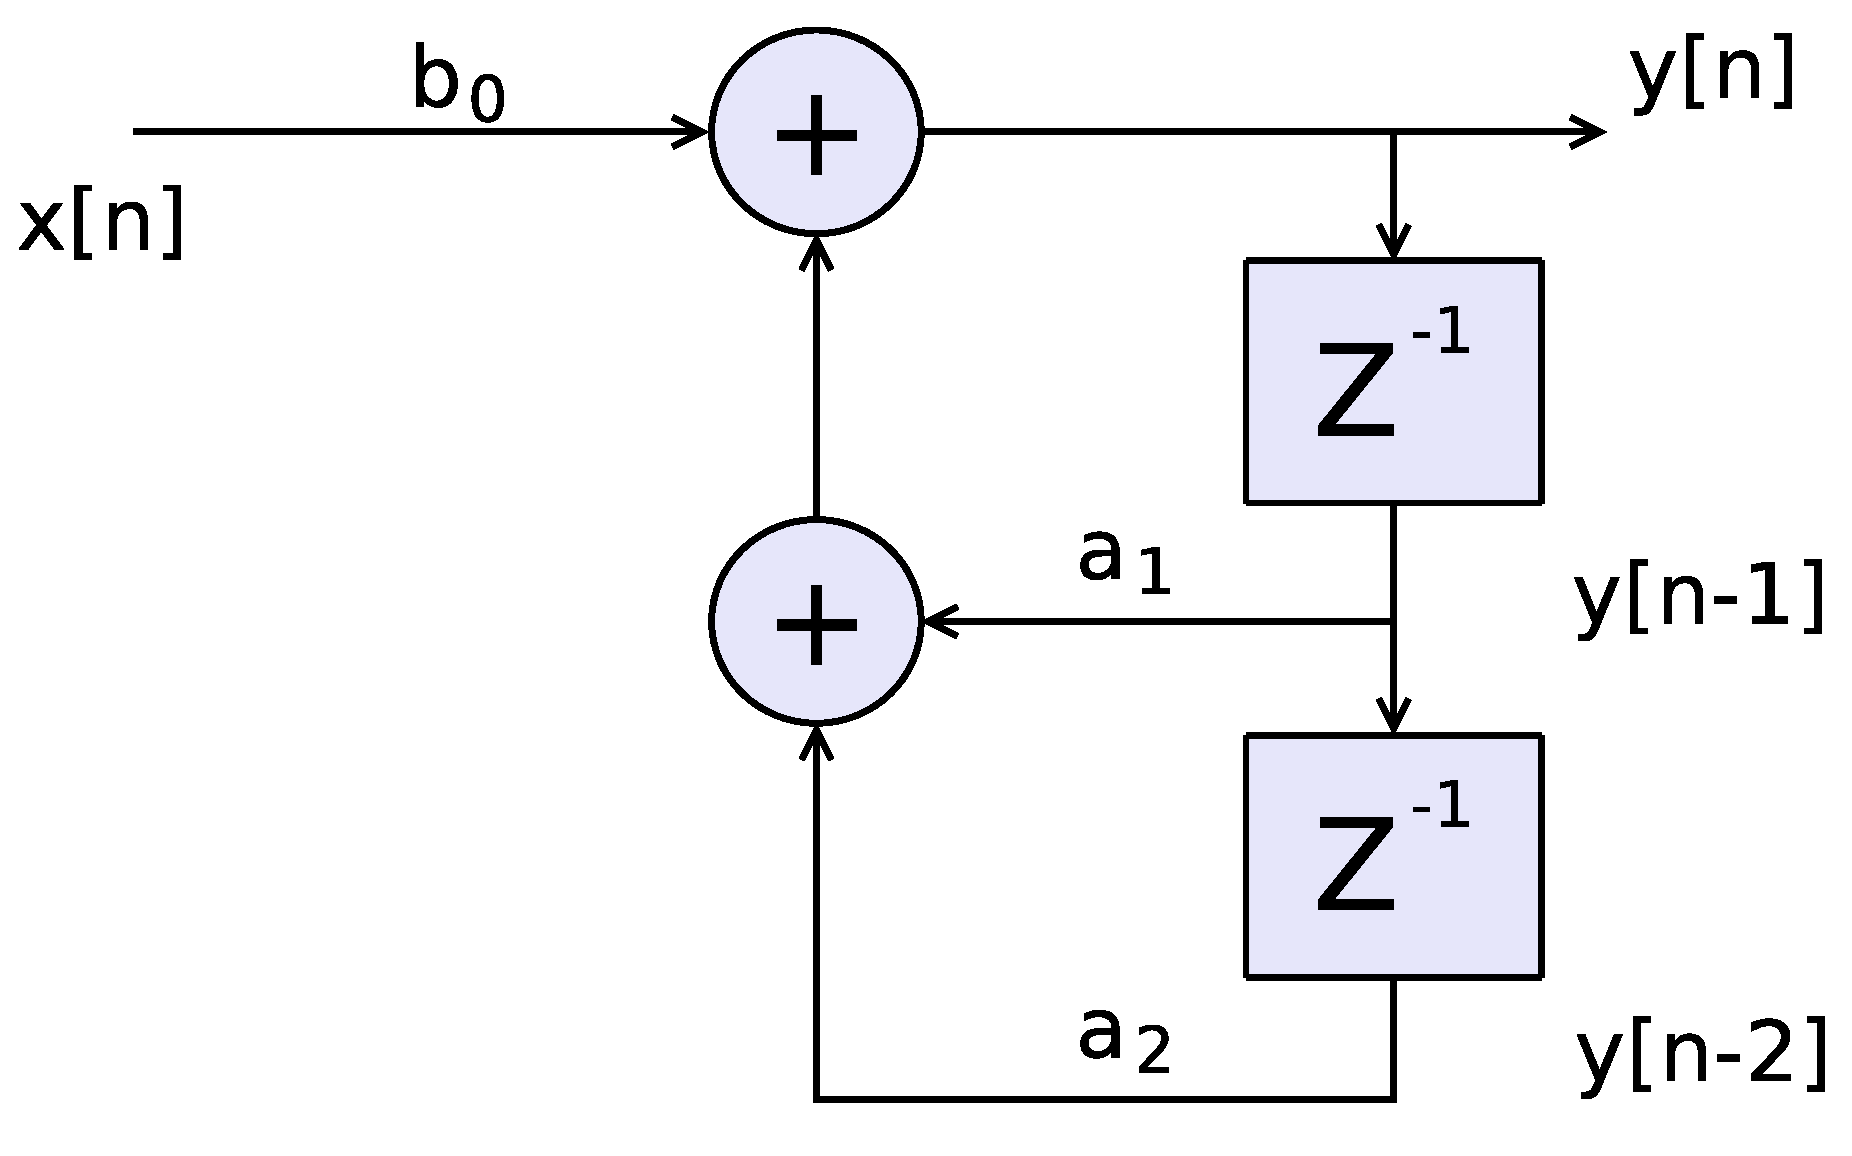
\includegraphics[width = 0.7\textwidth]{figs/ex2.eps}
   \end{figure}


\end{itemize}
\end{slide}

\begin{slide}{Diagrama de blocos}
\begin{itemize}
     \item Forma direta I
      %\begin{equation*}
       % \sum_{k = 0}^{N}a_ky[n-k]= \sum_{k = 0}^{M}b_kx[n-k], \qquad a_0=1
    %\end{equation*}
   \begin{figure}
       \centering
        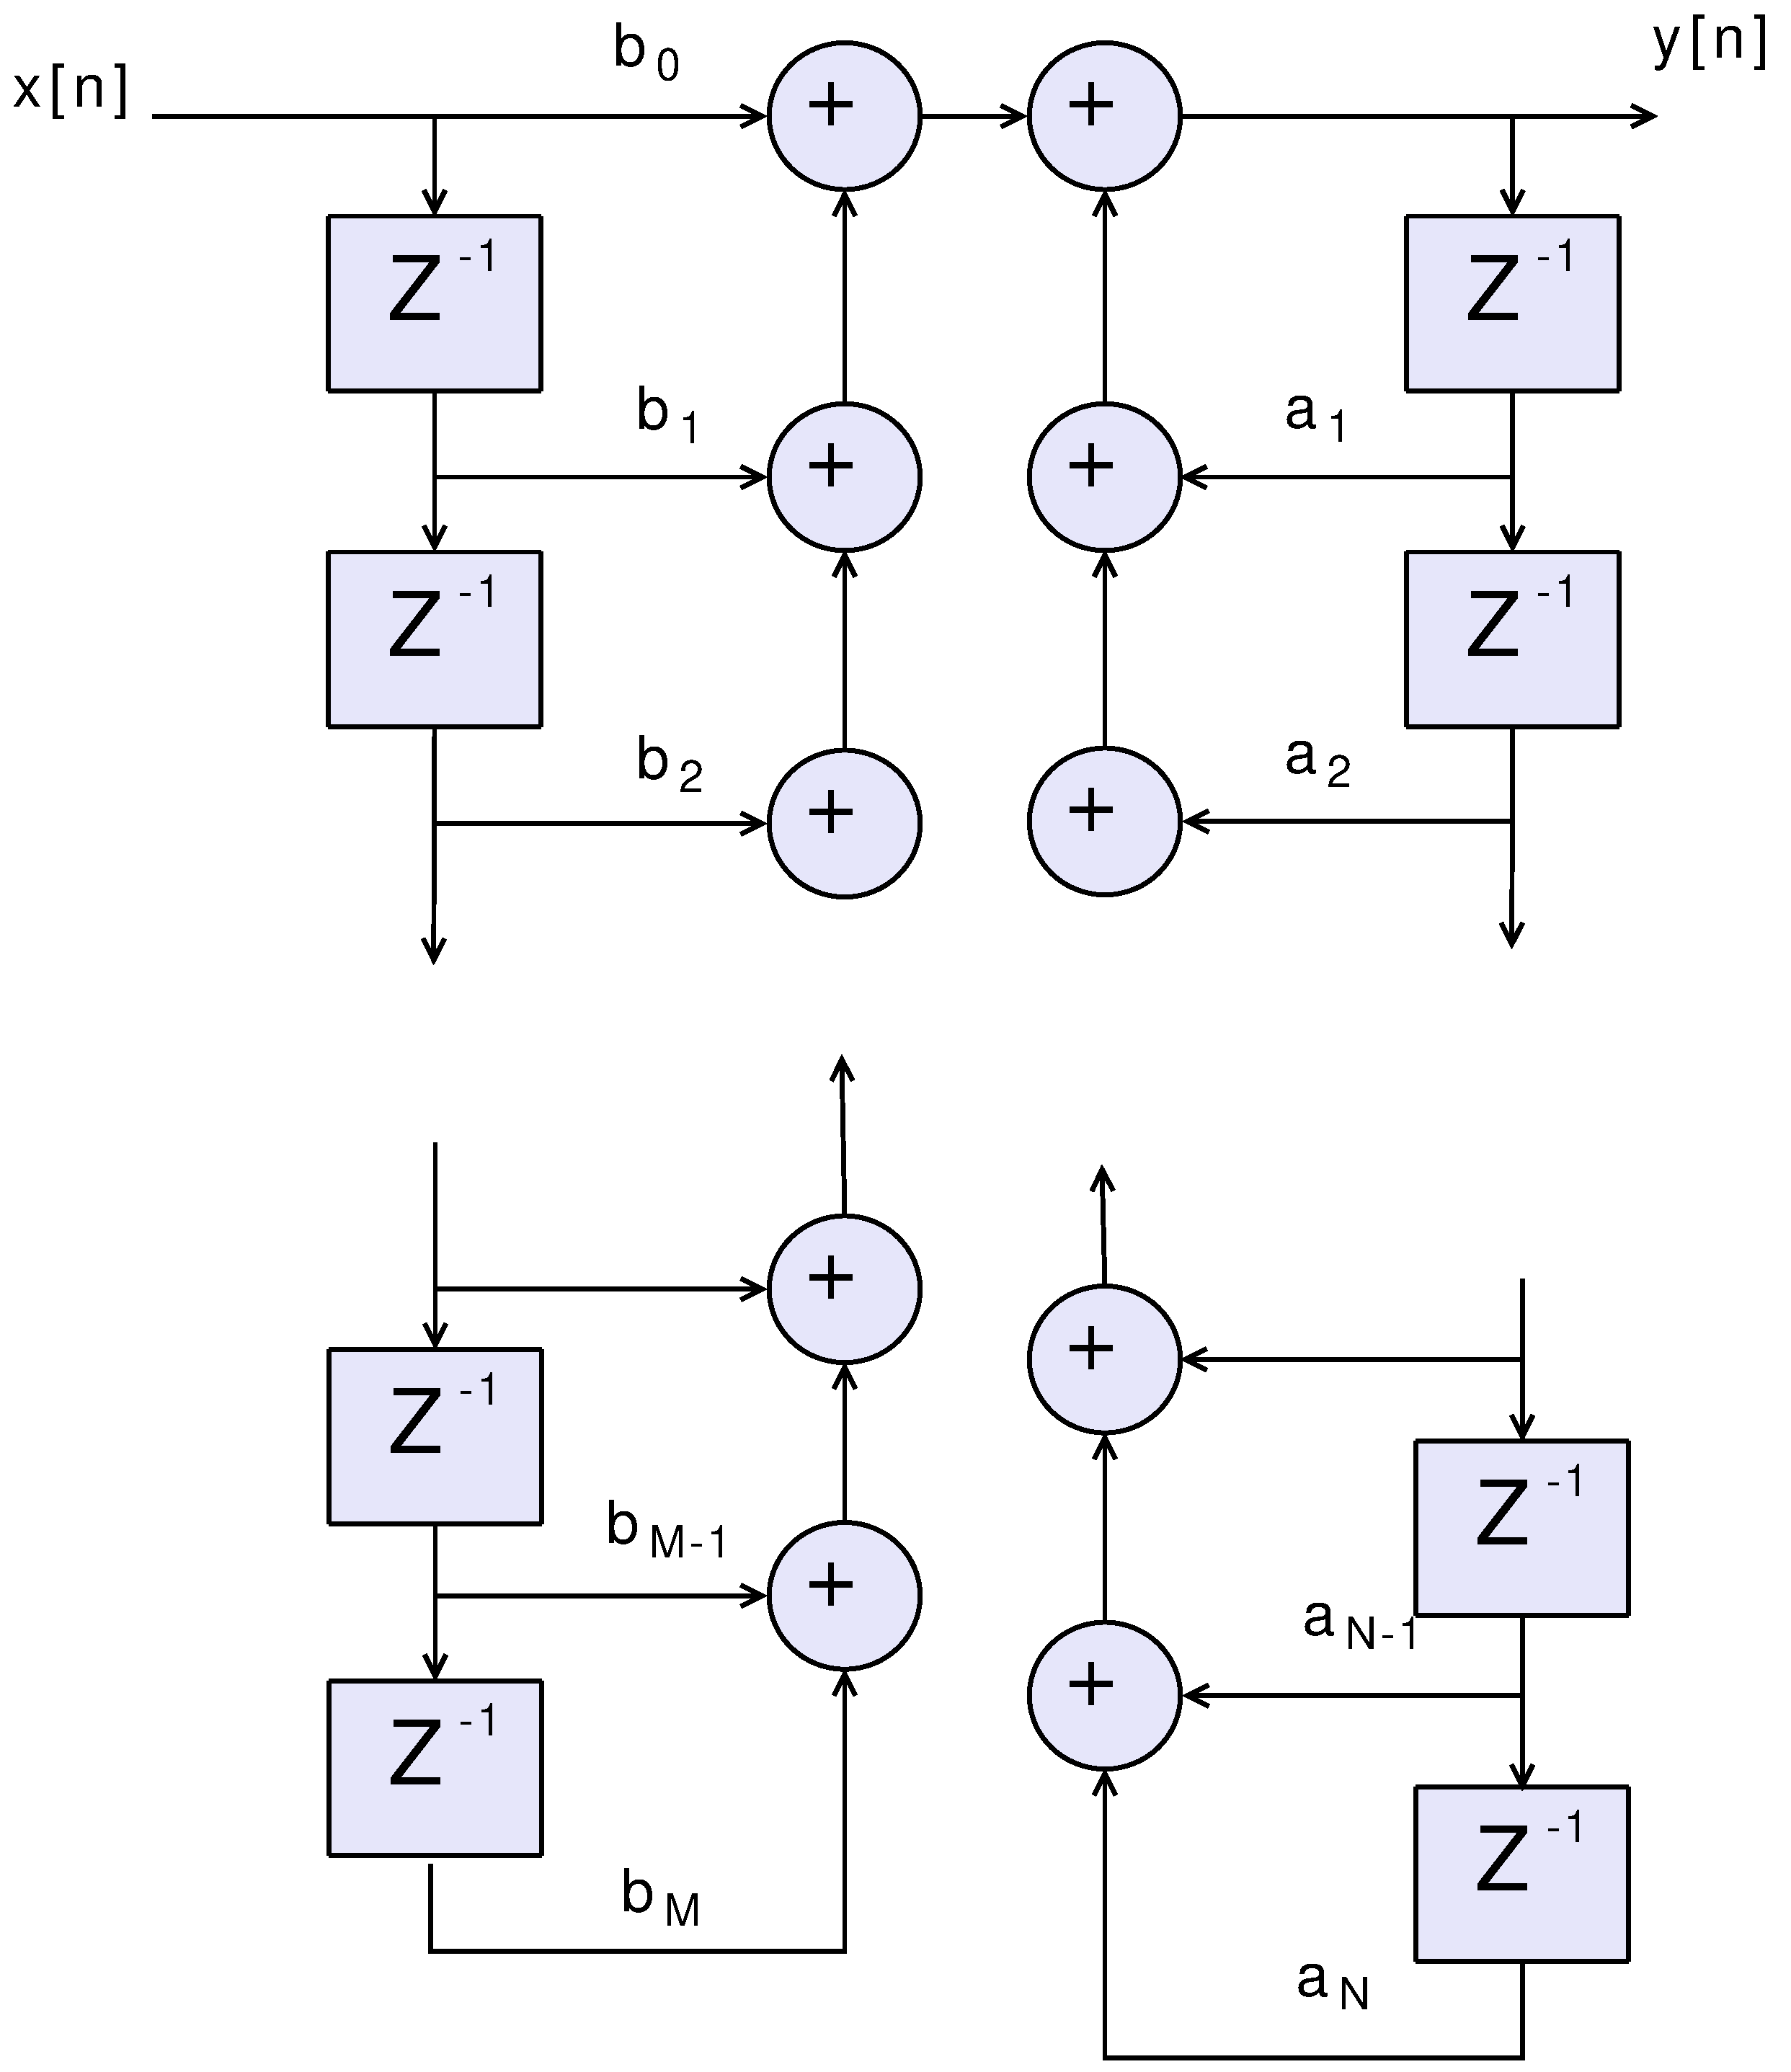
\includegraphics[width = 0.4\textwidth]{figs/fd1.eps}
        %\caption{Forma direta I.}
   \end{figure}
   

\end{itemize}
\end{slide}

\begin{slide}{Diagrama de blocos}
\begin{itemize}
     \item Forma direta II ou forma direta canônica
      %\begin{equation*}
       % \sum_{k = 0}^{N}a_ky[n-k]= \sum_{k = 0}^{M}b_kx[n-k], \qquad a_0=1
    %\end{equation*}
   \begin{figure}
       \centering
        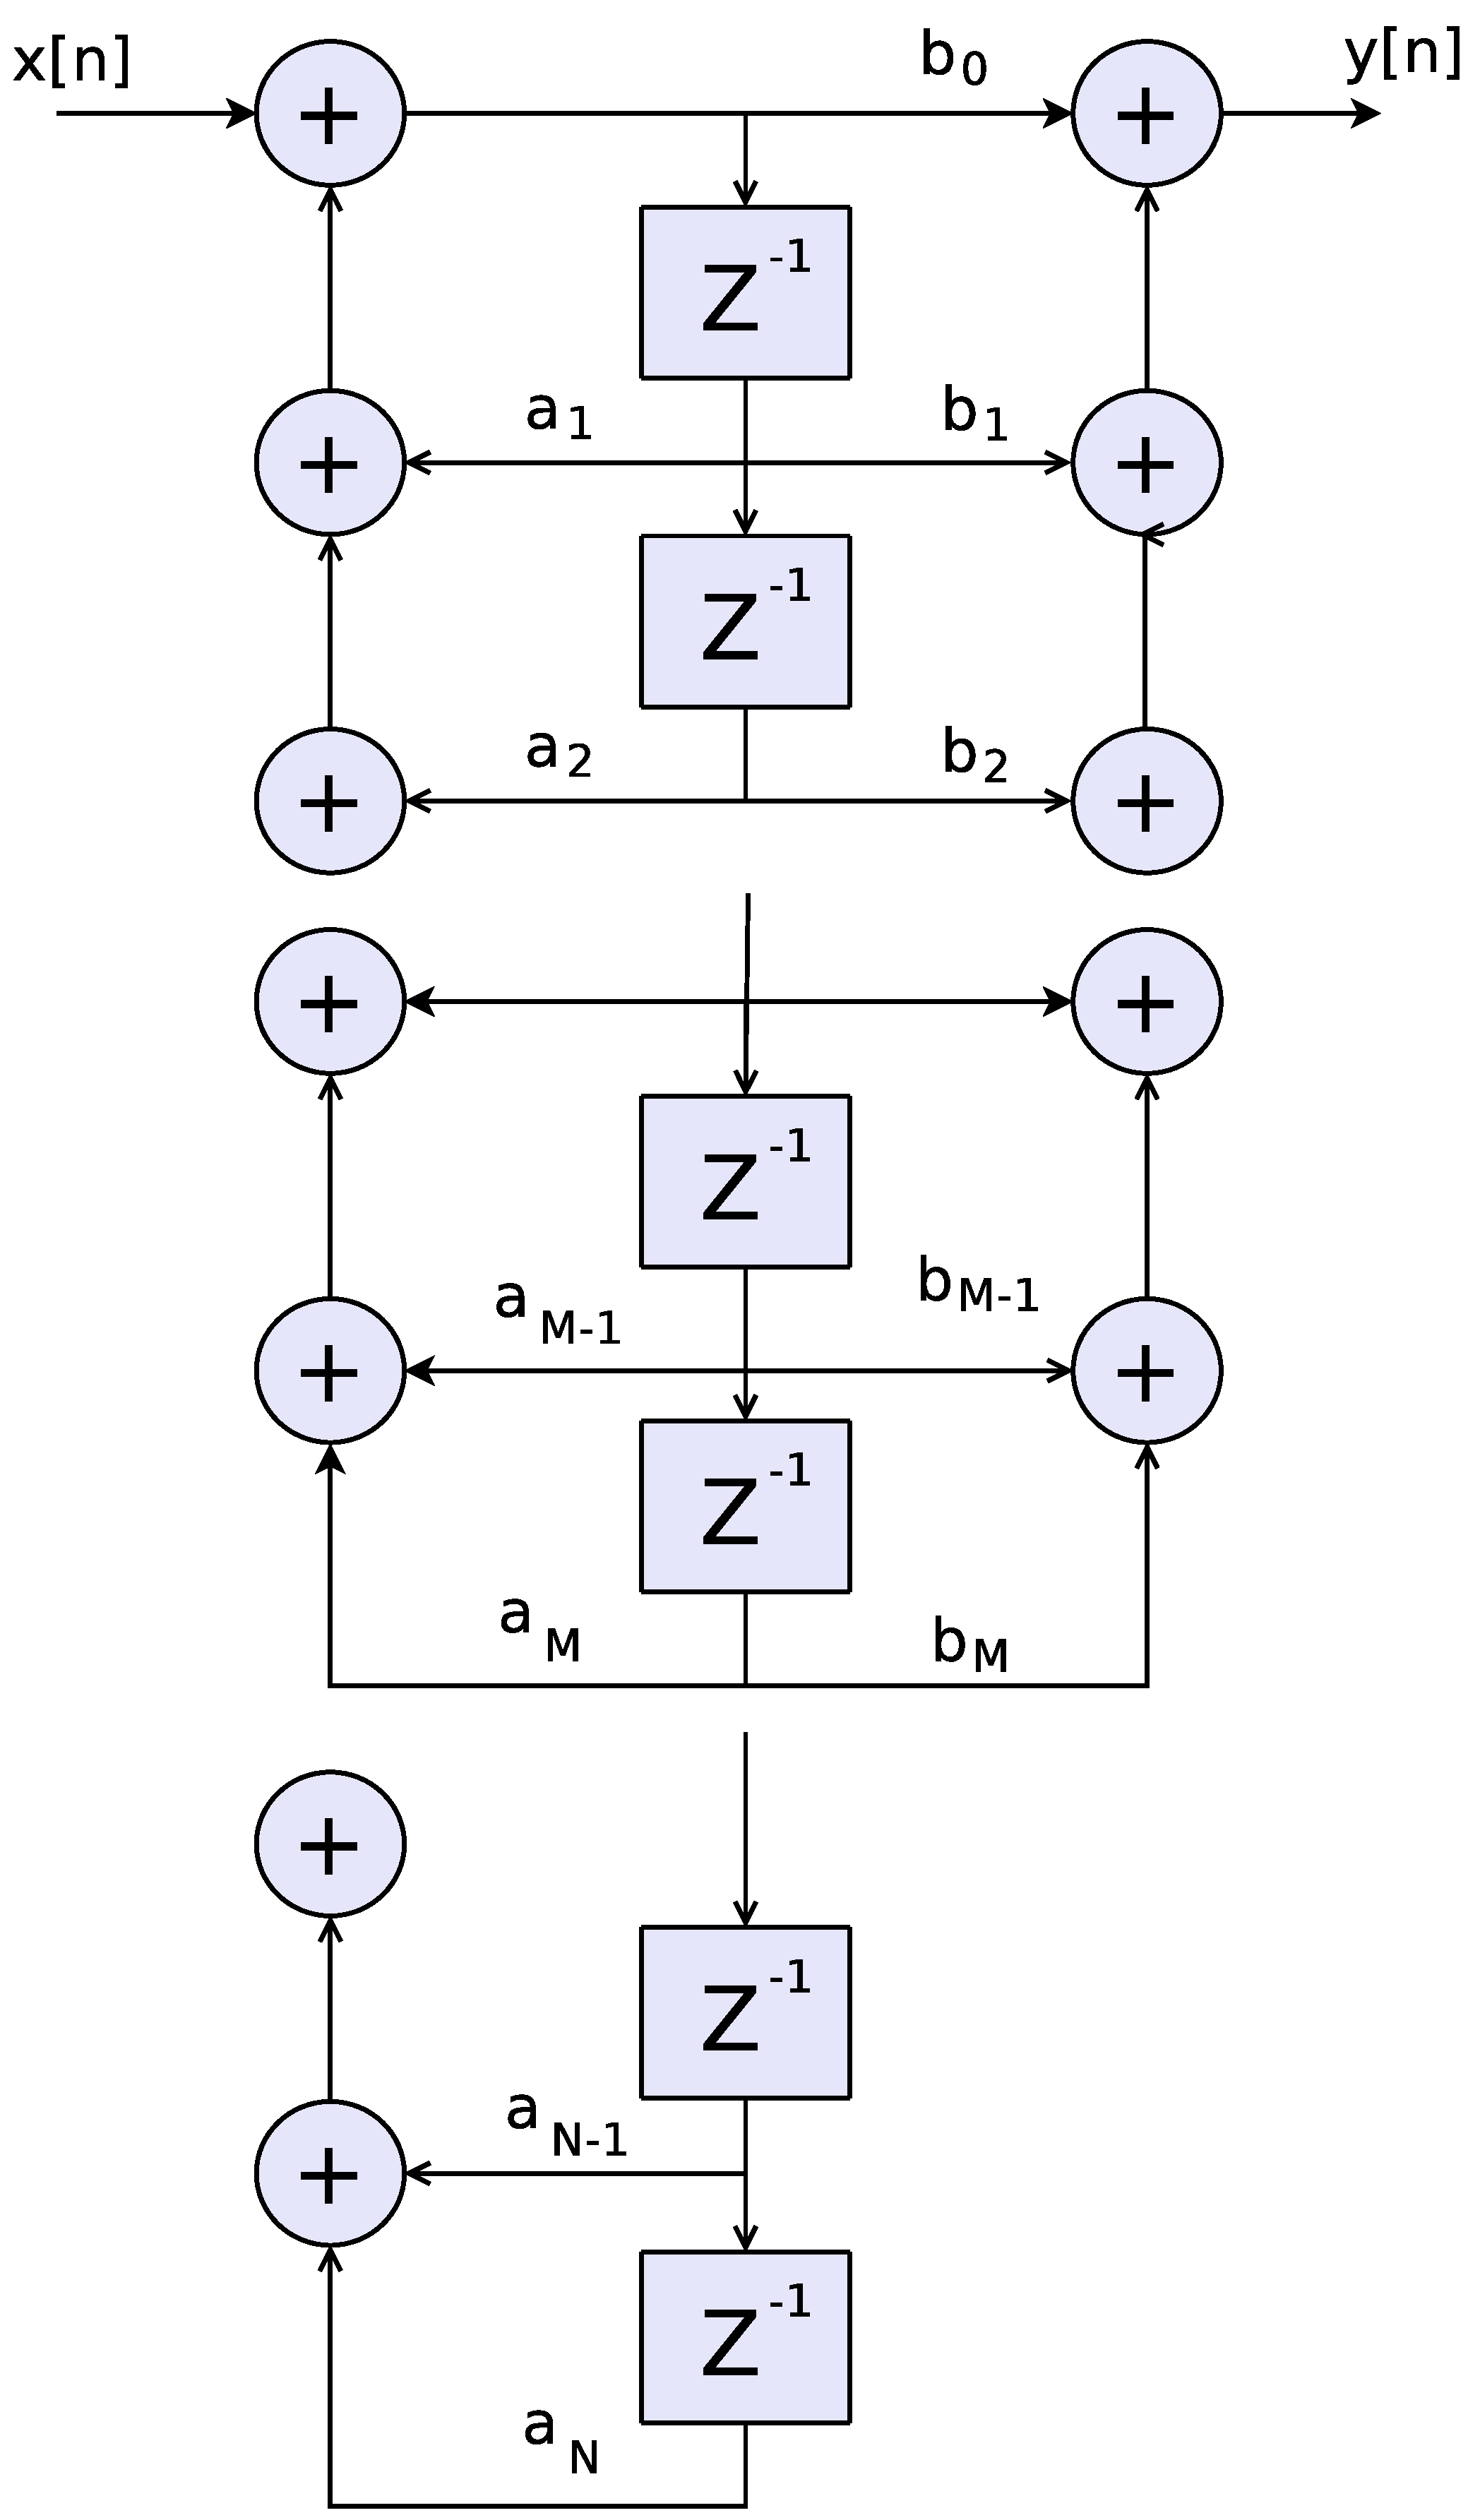
\includegraphics[width = 0.30\textwidth]{figs/fd2.eps}
        %\caption{Forma direta I.}
   \end{figure}
\end{itemize}
\end{slide}

\begin{slide}{Diagrama de blocos}
\begin{itemize}
   \item Ex3.: Considerando a função de transferência abaixo: (a) Represente em diagrama de blocos (Formas diretas I e II); e (b) Trace o diagrama de pólos e zeros, especificando a região de convergência (assuma que o sistema é causal).
    \begin{equation*}
        H(z)=\frac{1+2z^{-1}}{1-1,5z^{-1}+0,9z^{-2}}
    \end{equation*}
   %\item Ex.: represente em diagrama de blocos a eq. de diferenças 
   %\begin{equation*}
     %   y[n]= a_1y[n-1]+a_2y[n-2]+b_0x[n] 
    %\end{equation*}
\end{itemize}
\end{slide}

\section{Representação em grafo de fluxo de sinais}
\begin{slide}{Grafo de fluxo de sinais}    
    \begin{itemize}
   \item Elementos básicos:
   \begin{minipage}{\textwidth}
   \begin{minipage}{0.49\textwidth}
    \begin{itemize}
      \item Nó-fonte
      \item Nó-sorvedouro
      \item Nó-conexão
      \item Ramos orientados e ponderados
    \end{itemize}
   \end{minipage}
   \begin{minipage}{0.49\textwidth}
   \begin{figure}
       \centering
        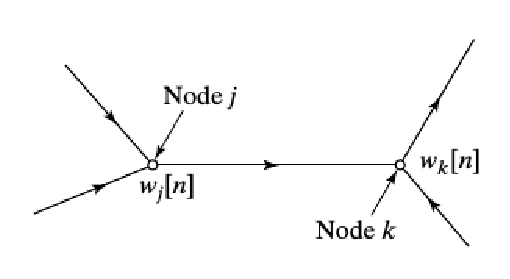
\includegraphics[width = 0.7\textwidth]{figs/graph}
        %\caption{Forma direta I.}
   \end{figure}
   \end{minipage}
   \end{minipage}
   \item Exemplo de diferentes representações para o mesmo sistema:
   \begin{figure}
       \centering
        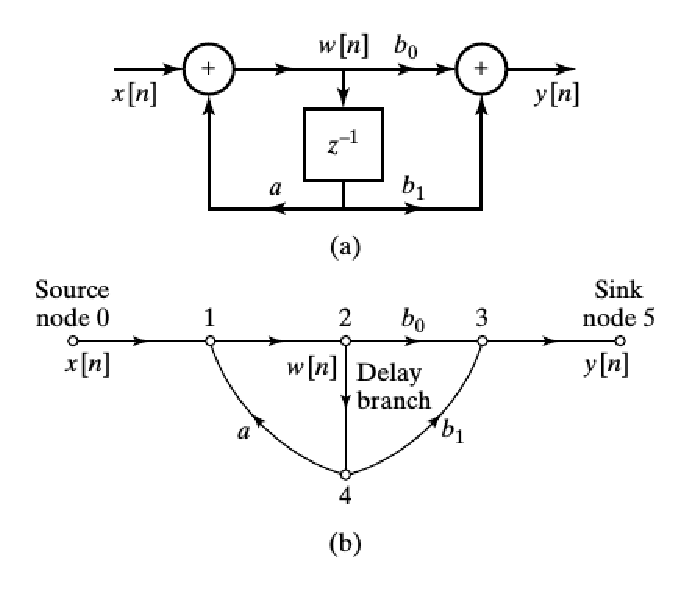
\includegraphics[width = 0.35\textwidth]{figs/block-graph-ex.eps}
        %\caption{Forma direta I.}
   \end{figure}
   %\item Ex. 4: Representar todos os sistemas dos exemplos anteriores em grafos de fluxo de sinal.
\end{itemize}
\end{slide}

\begin{slide}{Análise}
Exemplo: determinar a função de transferência, reposta ao impulso e a equação de diferenças
   \begin{figure}
       \centering
        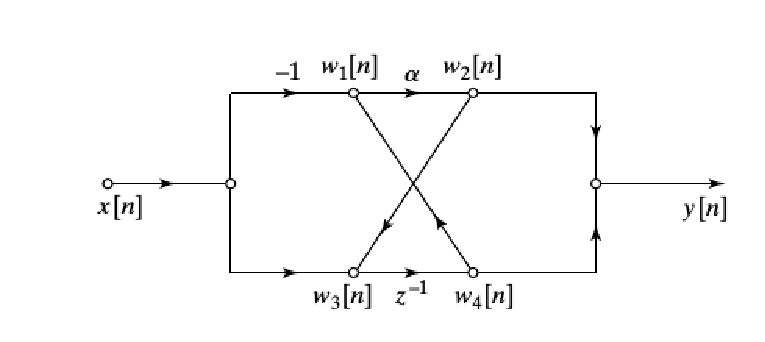
\includegraphics[width = 0.8\textwidth]{figs/no-std-form.eps}
        %\caption{Forma direta I.}
   \end{figure}
\end{slide}

\section{Estruturas básicas para sistemas IIR}
\begin{slide}{Formas diretas}
   \begin{itemize}
     \item Forma direta I
   \begin{figure}
       \centering
        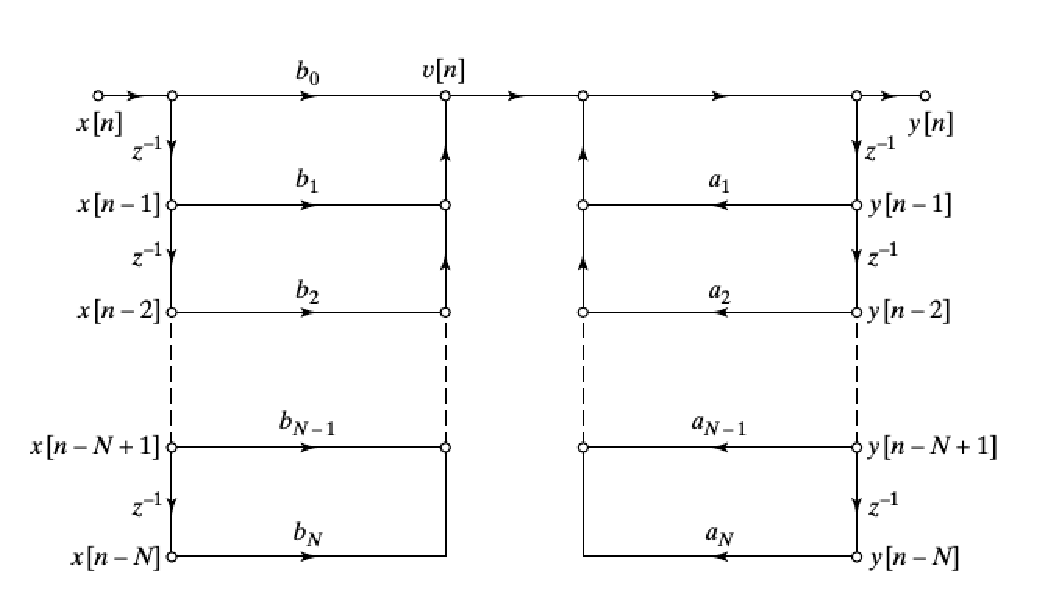
\includegraphics[width = 0.8\textwidth]{figs/f1.eps}
        %\caption{Forma direta I.}
   \end{figure}
  \end{itemize}
\end{slide}

\begin{slide}{Formas diretas}
   \begin{itemize}
     \item Forma direta II
   \begin{figure}
       \centering
        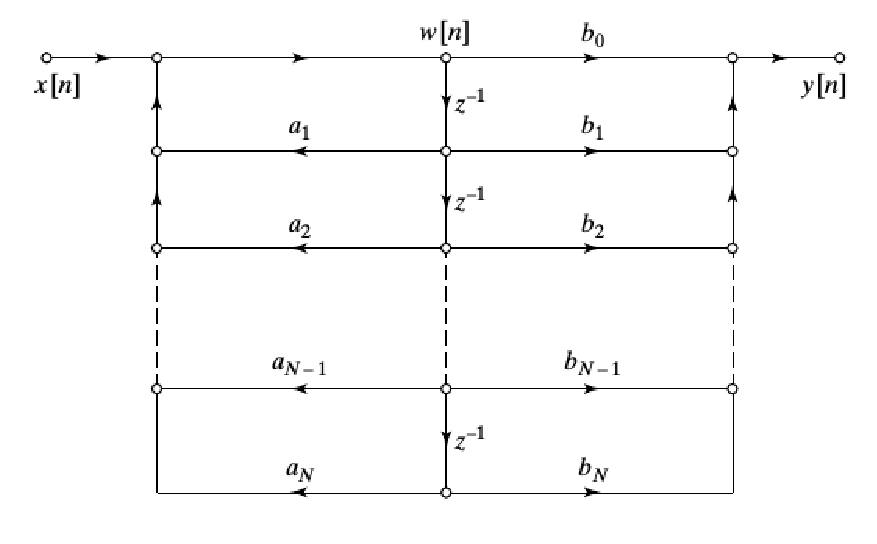
\includegraphics[width = 0.8\textwidth]{figs/f2.eps}
        %\caption{Forma direta I.}
   \end{figure}
  \end{itemize}
\end{slide}

\begin{slide}{Sistemas em cascata }
\begin{itemize}
   \item Cascata de sistemas de segunda ordem na forma direta II
   \begin{figure}
       \centering
        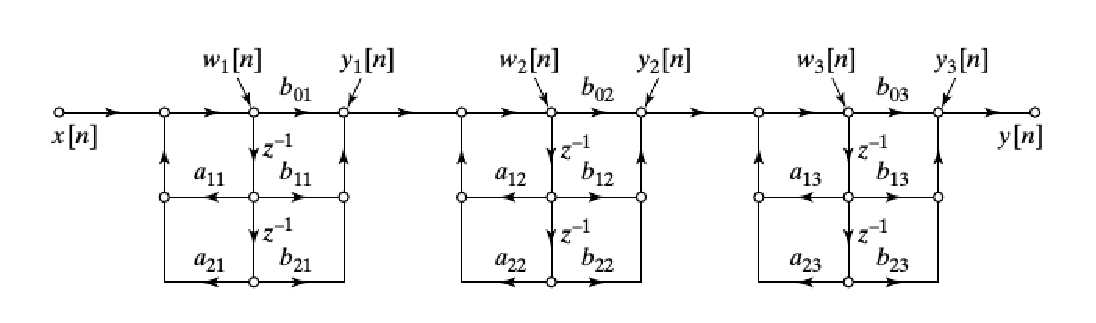
\includegraphics[width = 0.95\textwidth]{figs/cascade.eps}
        %\caption{Forma direta I.}
   \end{figure}
\end{itemize}
\end{slide}

\begin{slide}{Sistemas em paralelo}
\begin{itemize}
   \item Associação em paralelo de sistemas na forma direta II
   \begin{figure}
       \centering
        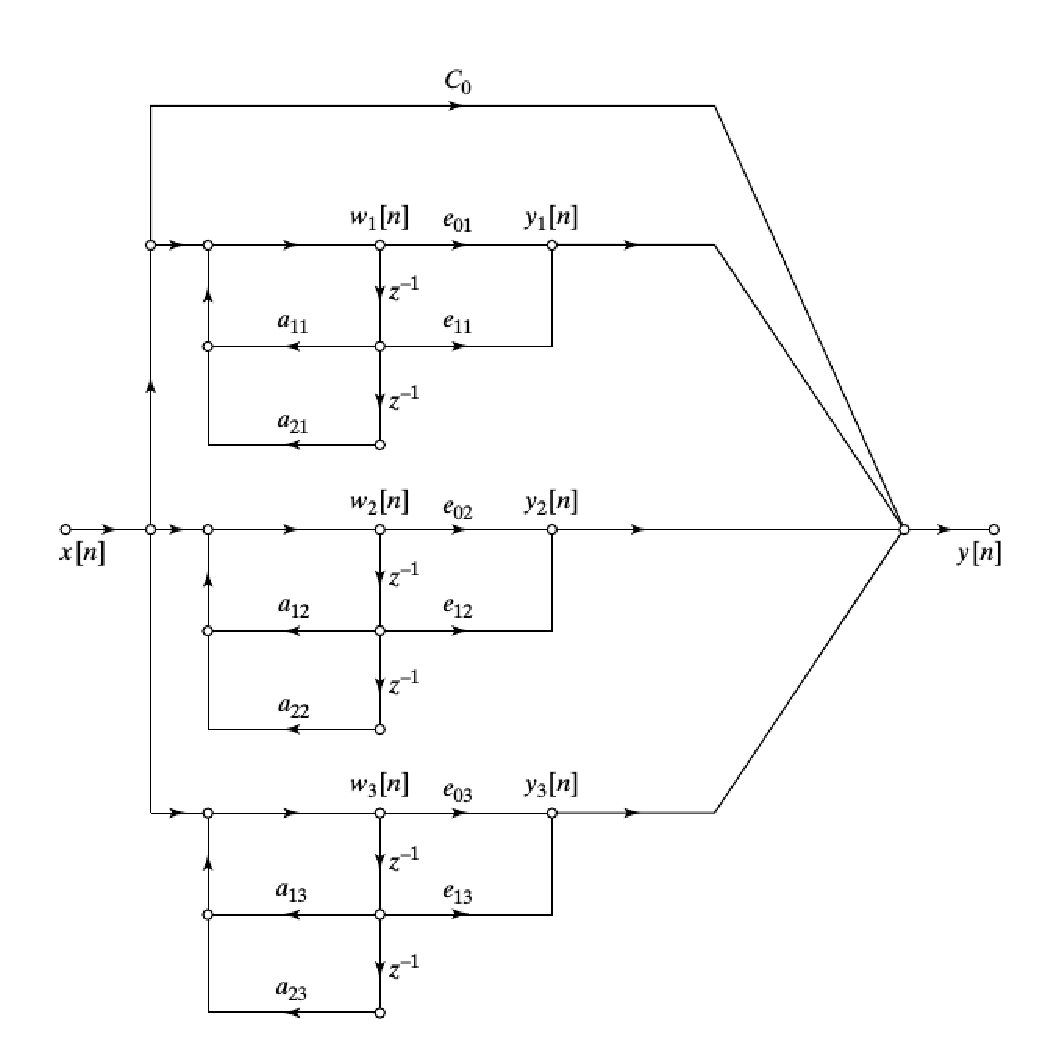
\includegraphics[width = 0.5\textwidth]{figs/parallel.eps}
        %\caption{Forma direta I.}
   \end{figure}
\end{itemize}
\end{slide}

\begin{slide}{Exemplos}
Encontrar implementações em cascata e em paralelo de sistemas de, no máximo primeira ordem, para o sistema:
	\begin{equation*}
		H(z) =\frac{1+2z^{-1}+z^{-2}}{1-0,75z^{-1}+0,125z^{-2}}
	\end{equation*}
\end{slide}

\section{Formas transpostas ou reversas}
\begin{slide}{Formas transpostas ou reversas}
	\begin{itemize}
		\item Procedimento para determinar a forma reversa de um grafo:
		\begin{itemize}
			\item Inverter as direções de todos os ramos
			\item Trocar entrada por saída
			\item Os ganhos de cada ramo são mantidos
		\end{itemize}
		\item Exemplo:
   			\begin{figure}
       				\centering
        			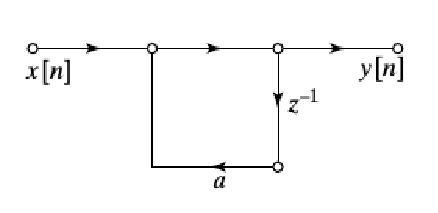
\includegraphics[width = 0.3\textwidth]{figs/transposed1.eps}
        			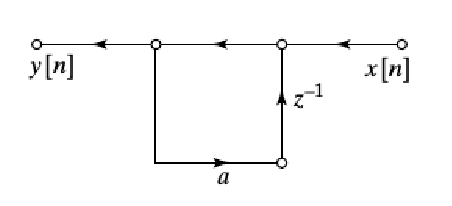
\includegraphics[width = 0.3\textwidth]{figs/transposed2.eps}
        			\includegraphics[width = 0.3\textwidth]{figs/transposed3.eps}
        			%\caption{Forma direta I.}
   			\end{figure}
	\end{itemize}
\end{slide}

\section{Estruturas básicas para sistemas FIR}
\begin{slide}{Estruturas básicas para sistemas FIR}
	\begin{itemize}
		\item Forma direta
   			\begin{figure}
       				\centering
        			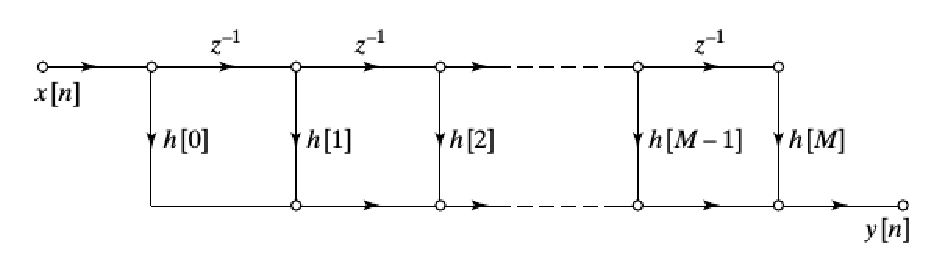
\includegraphics[width = 0.8\textwidth]{figs/firdirect.eps}
			\end{figure}
		\item Forma transposta
   			\begin{figure}
       				\centering
        			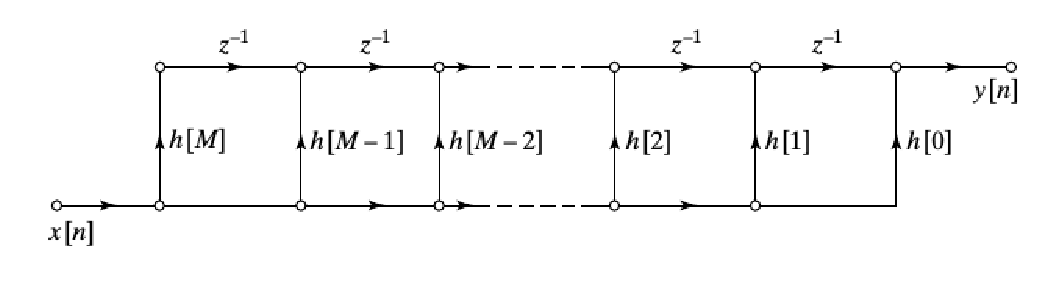
\includegraphics[width = 0.8\textwidth]{figs/firtransposed.eps}
			\end{figure}
	\end{itemize}
\end{slide}

\begin{slide}{Estruturas básicas para sistemas FIR}
	\begin{itemize}
		\item Organização em cascata
   			\begin{figure}
       				\centering
        			\includegraphics[width = 0.8\textwidth]{figs/fircascade.eps}
			\end{figure}
	\end{itemize}
\end{slide}

\begin{slide}{Estruturas básicas para sistemas FIR}
	\begin{itemize}
		\item Estruturas para sistemas de fase linear (ordem par)
   			\begin{figure}
       				\centering
        			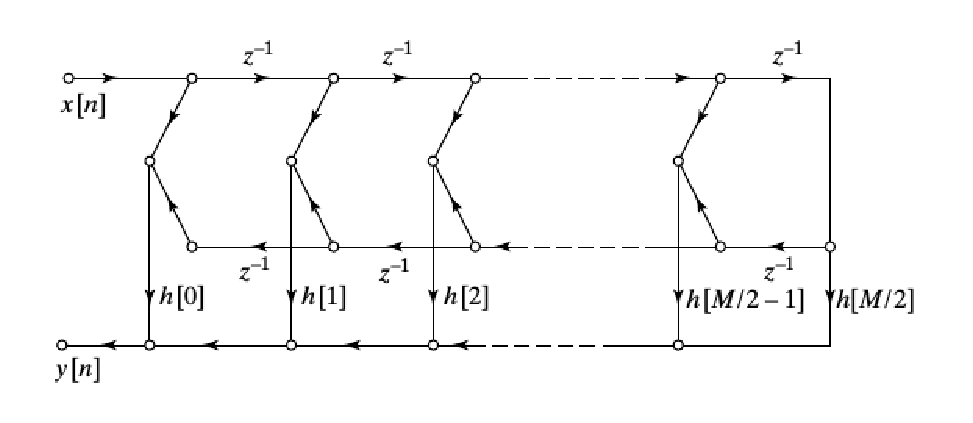
\includegraphics[width = 0.8\textwidth]{figs/firlinearphase1.eps}
			\end{figure}
	\end{itemize}
\end{slide}
\begin{slide}{Estruturas básicas para sistemas FIR}
	\begin{itemize}
		\item Estruturas para sistemas de fase linear (ordem ímpar)
   			\begin{figure}
       				\centering
        			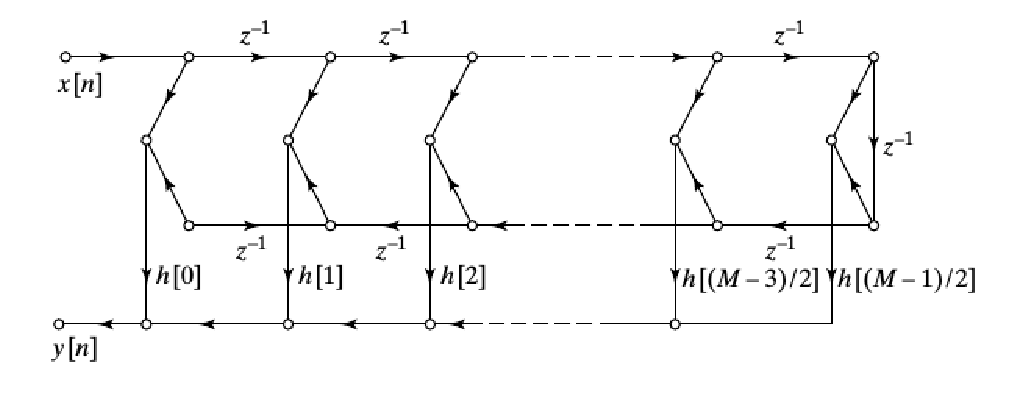
\includegraphics[width = 0.8\textwidth]{figs/firlinearphase2.eps}
			\end{figure}
	\end{itemize}
\end{slide}

\end{document}
